%% \documentclass[handout,t]{beamer} % HANDOUT
%% \documentclass[handout,notes=show,t]{beamer} % NOTES
\documentclass[t]{beamer} % SLIDES

\usetheme{ZipfR}
\usepackage{beamer-tools}

\input{lib/math}  % basic mathematical notation
\input{lib/stat}  % notation for probability theory and statistics
\input{lib/vector}% convenience macros for vectors and matrices

%%%
%%% local configuration adjustments
%%%

%%% You can change pre-defined colours here, override built-in macros from the
%%% style definition and standard library, as well as define macros needed by
%%% all local documents.

%%% e.g. adjust counterpoint (dark green) for data projectors where greens are
%%% far too bright, as well as green component of light colour and pure green
%%% (of course, it's a better solution to adjust the gamma settings of your monitor)
%%
%% \definecolor{counterpoint}{rgb}{.1, .3, 0}
%% \definecolor{light}{rgb}{.45, .3, .55}
%% \definecolor{puregreen}{rgb}{0, .35, 0}

%% ----- extra packages we need to load

\usepackage{tikz}
\usepackage{alltt}              % code examples with nicely formatted comments


%% ----- automatically show TOC reminder at beginning of each subsection
\AtBeginSubsection[]
{
  \begin{frame}
    \frametitle{Outline}
    \tableofcontents[current,currentsubsection]
  \end{frame}
}

%% ----- some useful macros for R examples

%% > plot(x,y)      \REM{this produces a scatterplot}
\newcommand{\REM}[2][\small]{\textsf{#1\color{primary}\# #2}}

%% nice colour for R output: \begin{Rout} .. \end{Rout}
%% -- ugly hack: I'm sure theres a better way to do this
\newenvironment{Rout}[1][\footnotesize]{%
  \begin{footnotesize}#1\color{dsmblue}\bfseries}{%
  \color{black}\mdseries\end{footnotesize}}

%% ----- other macros -----

%% \IV{condition} ... indicator variable
\newcommand{\IV}[1]{I_{[#1]}}

%% \dpi ... integration over pi
\newcommand{\dpi}[0]{\dX{\pi}} % local adjustments to configuration and macros

%%%%%%%%%%%%%%%%%%%%%%%%%%%%%%%%%%%%%%%%%%%%%%%%%%%%%%%%%%%%%%%%%%%%%%
%% Titlepage

\title[LNRE models]{LNRE models of type-token distributions}
\subtitle{}
\author[Stefan Evert]{Stefan Evert\\ FAU Erlangen-Nürnberg}
\date[Würzburg | 3 Sep 2018]{\small Kallimachos II\\Würzburg, 3 Sep 2018}

\begin{document}

\pgfdeclareimage[width=30mm]{kallimachos-logo}{img/logo_kallimachos}
\logo{\pgfuseimage{kallimachos-logo}}

\frame{\titlepage}
\hideLogo{}
%% \AtBeginSubsection[]{}

%%%%%%%%%%%%%%%%%%%%%%%%%%%%%%%%%%%%%%%%%%%%%%%%%%%%%%%%%%%%%%%%%%%%%%%%

\section*{Outline}
\frame{ 
  \frametitle{Outline}
  \tableofcontents
}

%%%%%%%%%%%%%%%%%%%%%%%%%%%%%%%%%%%%%%%%%%%%%%%%%%%%%%%%%%%%%%%%%%%%%%%%
\section{Introduction}

%%%%%%%%%%%%%%%%%%%%%%%%%%%%%%%%%%%%%%%%%%%%%%%%%%%%%%%%%%%%%%%%%%%%%%%%
\subsection{Applications}

\begin{frame}
  \frametitle{Applications of type-token statistics}

  \begin{itemize}
  \item How many words did Shakespeare know?
  \item What is the coverage of my treebank grammar on big data?
  \item How many typos are there on the Internet?
  \item Is \emph{-ness} more productive than \emph{-ity} in English?
  \item Are there differences in the productivity of nominal compounds between academic writing and novels?
  \item Does Dickens use a more complex vocabulary than Rowling?
  \item Can a decline in lexical complexity predict Alzheimer's disease?
  \item How frequent is a hapax legomenon from the Brown corpus?
  \item What is appropriate smoothing for my n-gram model?
  \item Who wrote the Bixby letter, Lincoln or Hay?
  \item How many different species of \ldots\ are there? \citep{Brainerd:82}
  \end{itemize}
\end{frame}

\begin{frame}
  \frametitle{Applications of type-token statistics}

  \begin{itemize}
  \item 
  \item \counterpoint{coverage estimates}
  \item
  \item
  \item \counterpoint{productivity}\\\rule{0mm}{1ex}
  \item \counterpoint{lexical complexity \& stylometry}
  \item 
  \item \counterpoint{prior \& posterior distribution}
  \item 
  \item \counterpoint{unexpected applications}
  \item 
  \end{itemize}
\end{frame}

%%%%%%%%%%%%%%%%%%%%%%%%%%%%%%%%%%%%%%%%%%%%%%%%%%%%%%%%%%%%%%%%%%%%%%%%
\subsection{Notation \& basic concepts}

\newcommand{\TC}[1]{\counterpoint{\emph{#1}}}
\newcommand{\TL}[1]{\light{\emph{#1}}}
\newcommand<>{\TA}[1]{\light{\counterpoint#2{\emph{#1}}}}

\begin{frame}
  \frametitle{Tokens \& types}

  our sample: \TC{recently}, \TC{very}, \TC{not}, \TC{otherwise}, \TC{much}, \TC{very},
  \TC{very}, \TC{merely}, \TC{not}, \TC{now}, \TC{very}, \TC{much},
  \TC{merely}, \TC{not}, \TC{very}

  \begin{itemize}
  \item $N = 15$: number of \hh{tokens} = sample size
  \item $V = 7$: number of distinct \hh{types} = \h{vocabulary size}\\
    (\TC{recently}, \TC{very}, \TC{not}, \TC{otherwise}, \TC{much}, \TC{merely}, \TC{now})
  \end{itemize}

  \onslide<2->
  \begin{columns}[c]
    \begin{column}{5cm}
      \centering
      \h{type-frequency list}

      \begin{tabular}{l|c}
        $w$ & $f_w$ \\
        \hline
        \TC{recently} & 1 \\ 
        \TC{very}     & 5 \\
        \TC{not}      & 3 \\ 
        \TC{otherwise}& 1 \\ 
        \TC{much}     & 2 \\ 
        \TC{merely}   & 2 \\ 
        \TC{now}      & 1 
      \end{tabular}
    \end{column}
    \begin{column}{5cm}
      
    \end{column}
  \end{columns}
\end{frame}

\begin{frame}
  \frametitle{Zipf ranking}

  our sample: \TC{recently}, \TC{very}, \TC{not}, \TC{otherwise}, \TC{much}, \TC{very},
  \TC{very}, \TC{merely}, \TC{not}, \TC{now}, \TC{very}, \TC{much},
  \TC{merely}, \TC{not}, \TC{very}

  \begin{itemize}
  \item $N = 15$: number of \hh{tokens} = sample size
  \item $V = 7$: number of distinct \hh{types} = \h{vocabulary size}\\
    (\TC{recently}, \TC{very}, \TC{not}, \TC{otherwise}, \TC{much}, \TC{merely}, \TC{now})
  \end{itemize}

  \begin{columns}[c]
    \begin{column}{5cm}
      \centering
      \h{Zipf ranking}

      \begin{tabular}{l|c|c}
        $w$ & $r$ & $f_r$ \\
        \hline
        \TL{very}     & 1 & 5 \\
        \TL{not}      & 2 & 3 \\ 
        \TL{merely}   & 3 & 2 \\ 
        \TL{much}     & 4 & 2 \\ 
        \TL{now}      & 5 & 1 \\
        \TL{otherwise}& 6 & 1 \\ 
        \TL{recently} & 7 & 1 
      \end{tabular}
    \end{column}
    \begin{column}{5cm}
      \visible<2->{\includegraphics[width=45mm]{../plots/tutorial_tfl}}
    \end{column}
  \end{columns}
\end{frame}

\begin{frame}
  \frametitle{A realistic Zipf ranking: the Brown corpus}

  \gap
  \begin{scriptsize}
    \begin{tabular}{|r|r|l||r|r|l|}
      \hline
      \multicolumn{3}{|c||}{\hh{top frequencies}} & \multicolumn{3}{c|}{\hh{bottom frequencies}}\\
      \hline
      \textbf{\textit{r}} & \multicolumn{1}{c|}{\textbf{\textit{f}}} & \textbf{word} & \textbf{rank range} & \multicolumn{1}{c|}{\textbf{\textit{f}}} & \textbf{randomly selected examples}\\
      \hline
       1 & 69836 & the   &   7731 -- \phantom{0}8271 & 10 &    schedules, polynomials, bleak \\ 
       2 & 36365 & of    &   8272 -- \phantom{0}8922 &  9 &          tolerance, shaved, hymn \\ 
       3 & 28826 & and   &   8923 -- \phantom{0}9703 &  8 & decreased, abolish, irresistible \\ 
       4 & 26126 & to    &   9704 -- 10783 &  7 &        immunity, cruising, titan \\ 
       5 & 23157 & a     &  10784 -- 11985 &  6 &     geographic, lauro, portrayed \\ 
       6 & 21314 & in    &  11986 -- 13690 &  5 &     grigori, slashing, developer \\ 
       7 & 10777 & that  &  13691 -- 15991 &  4 &       sheath, gaulle, ellipsoids \\ 
       8 & 10182 & is    &  15992 -- 19627 &  3 &         mc, initials, abstracted \\ 
       9 &  9968 & was   &  19628 -- 26085 &  2 &         thar, slackening, deluxe \\ 
      10 &  9801 & he    &  26086 -- 45215 &  1 &  beck, encompasses, second-place \\ 
      \hline
    \end{tabular}
  \end{scriptsize}
\end{frame}

\begin{frame}
  \frametitle{A realistic Zipf ranking: the Brown corpus}

  \ungap[1]
  \begin{center}
    \only<beamer:1| handout:0>{\includegraphics[height=7.5cm]{../plots/tutorial_brown_tfl}}%
    \only<beamer:2| handout:1>{\includegraphics[height=7.5cm]{../plots/tutorial_brown_tfl_log}}%
  \end{center}
\end{frame}

\begin{frame}
  \frametitle{Frequency spectrum}

  \ungap[1.5]
  \begin{itemize}
  \item pool types with $f = 1$ (\primary{hapax legomena}), types with $f = 2$ (\primary{dis legomena}), \ldots, $f = m$, \ldots
  \item $V_1 = 3$: number of hapax legomena (\emph{now, otherwise, recently})
  \item $V_2 = 2$: number of dis legomena (\emph{merely, much})
  \item general definition: $V_m = \abs{\setdef{w}{f_w = m}}$
  \end{itemize}
  
  \begin{columns}[c]
    \begin{column}{35mm}
      \centering
      \textbf{Zipf ranking}

      \begin{tabular}{l|c|c}
        $w$ & $r$ & $f_r$ \\
        \hline
        \TL{very}     & 1 & 5 \\
        \TL{not}      & 2 & 3 \\ 
        \TL{merely}   & 3 & 2 \\ 
        \TL{much}     & 4 & 2 \\ 
        \TL{now}      & 5 & 1 \\
        \TL{otherwise}& 6 & 1 \\ 
        \TL{recently} & 7 & 1 
      \end{tabular}
    \end{column}
    \begin{column}{25mm}
      \centering
      \h{frequency\\ spectrum}

      \begin{tabular}{c|c}
        $m$ & $V_m$ \\
        \hline
        1 & 3 \\
        2 & 2 \\
        3 & 1 \\
        5 & 1
      \end{tabular}
    \end{column}
    \begin{column}{5cm}
      \visible<2->{\includegraphics[width=45mm]{../plots/tutorial_spc}}
    \end{column}
  \end{columns}

\end{frame}

\begin{frame}
  \frametitle{A realistic frequency spectrum: the Brown corpus}

  \ungap[1]
  \begin{center}
    \includegraphics[height=7.5cm]{../plots/tutorial_brown_spc}%
  \end{center}
\end{frame}

\begin{frame}
  \frametitle{Vocabulary growth curve}
  
    our sample: \TA<1->{recently}, \TA<2->{very}, \TA<2->{not}, \TA<3->{otherwise}, \TA<3->{much}, \TA<3->{very},
  \TA<3->{very}, \TA<4->{merely}, \TA<4->{not}, \TA<4->{now}, \TA<4->{very}, \TA<4->{much},
  \TA<5->{merely}, \TA<5->{not}, \TA<5->{very}

  \begin{columns}[c]
    \begin{column}{6cm}
      \begin{itemize}
      \item<1-> $N = 1$, $V(N) = 1$, $V_1(N) = 1$
      \item<2-> $N = 3$, $V(N) = 3$, $V_1(N) = 3$
      \item<3-> $N = 7$, $V(N) = 5$, $V_1(N) = 4$
      \item<4-> $N = 12$, $V(N) = 7$, $V_1(N) = 4$
      \item<5-> $N = 15$, $V(N) = 7$, $V_1(N) = 3$
      \end{itemize}
    \end{column}
    \begin{column}{5cm}
      \visible<6->{\includegraphics[width=5cm]{../plots/tutorial_vgc}}%
    \end{column}
  \end{columns}

\end{frame}

\begin{frame}
  \frametitle{A realistic vocabulary growth curve: the Brown corpus}

  \ungap[1]
  \begin{center}
    \includegraphics[height=6.5cm]{../plots/tutorial_brown_vgc}%
  \end{center}
\end{frame}

\begin{frame}
  \frametitle{Vocabulary growth in authorship attribution}

  \begin{itemize}
  \item Authorship attribution by n-gram tracing applied to the case of the Bixby letter \citep{Grieve:etc:18}
  \item Word or character n-grams in disputed text are compared against large ``training'' corpora from candidate authors
  \end{itemize}

  \begin{center}
    \includegraphics[width=7cm]{img/GrieveEtc2018_fig1}
  \end{center}
\end{frame}

%%%%%%%%%%%%%%%%%%%%%%%%%%%%%%%%%%%%%%%%%%%%%%%%%%%%%%%%%%%%%%%%%%%%%%%%
\subsection{Productivity \& lexical diversity}

\begin{frame}
  \frametitle{Measuring morphological productivity}
  \framesubtitle{example from \citet{Evert:Luedeling:01}}
  
  \centering
  \only<beamer:1| handout:1>{\includegraphics[width=11cm]{../plots/EL2001_vgc_bar_sam_oes}}%
  \only<beamer:2| handout:0>{\includegraphics[width=11cm]{../plots/EL2001_vgc_bar_sam_oes_extrap}}%
\end{frame}

\begin{frame}
  \frametitle{Quantitative measures of productivity}
  \framesubtitle{\citep{Tweedie:Baayen:98,Baayen:01}}

  \footnotesize
  \begin{columns}[c]
        \begin{column}{6cm}
      \ungap[1.2]
      \begin{itemize}
      \item Baayen's (\citeyear{Baayen:91}) productivity index $\mathcal{P}$\\
        (slope of vocabulary growth curve)
        \[
        \mathcal{P} = \frac{V_1}{N}
        \]
      \item TTR = type-token ratio
        \[
        \text{TTR} = \frac{V}{N}
        \]
      \item Population size
        \[
        S = \lim_{N \to \infty} V(N)
        \]
      \item Herdan's law (\citeyear{Herdan:64})
        \[
        C = \frac{\log V}{\log N}
        \]
      \end{itemize}
    \end{column}
    \begin{column}{6cm}
      \begin{itemize}
      \item<2-> \citet{Yule:44} /  Simpson (1949) 
        \[
          K = 10\,000\cdot \frac{\sum_m m^2 V_m - N}{N^2}
        \]
      \item<2-> Guiraud (1954)
        \[
          R = \frac{V}{\sqrt{N}}
        \]
      \item<2-> \citet{Sichel:75}
        \[
          S = \frac{V_2}{V}
        \]
      \item<2-> Honoré (1979)
        \[
          H = \frac{\log N}{1 - \frac{V_1}{V}}
        \]
      \end{itemize}
    \end{column}
  \end{columns}  
\end{frame}

\begin{frame}[c]
  \frametitle{Productivity measures for bare singulars in the BNC}
  %% \framesubtitle{}

  \begin{columns}[c]
    \begin{column}{6cm}
      \centering
      \begin{tabular}{c@{$\qquad$}r@{$\qquad$}r}
        \toprule
        &    spoken &   written \\
        \midrule
        $V$     &  2,039 & 12,876 \\
        $N$     &  6,766 & 85,750 \\
        \midrule
        $K$     &    86.84 &    28.57 \\
        $R$     &    24.79 &    43.97 \\
        $S$     &     0.13 &     0.15 \\
        $C$     &     0.86 &     0.83 \\
        $\mathcal{P}$     &     0.21 &     0.08 \\
        TTR   &     0.301 &     0.150 \\
        pop.\ $S$ & 15,958 & 36,874 \\
        \bottomrule
      \end{tabular}
    \end{column}
    \begin{column}{6cm}
      \visible<2->{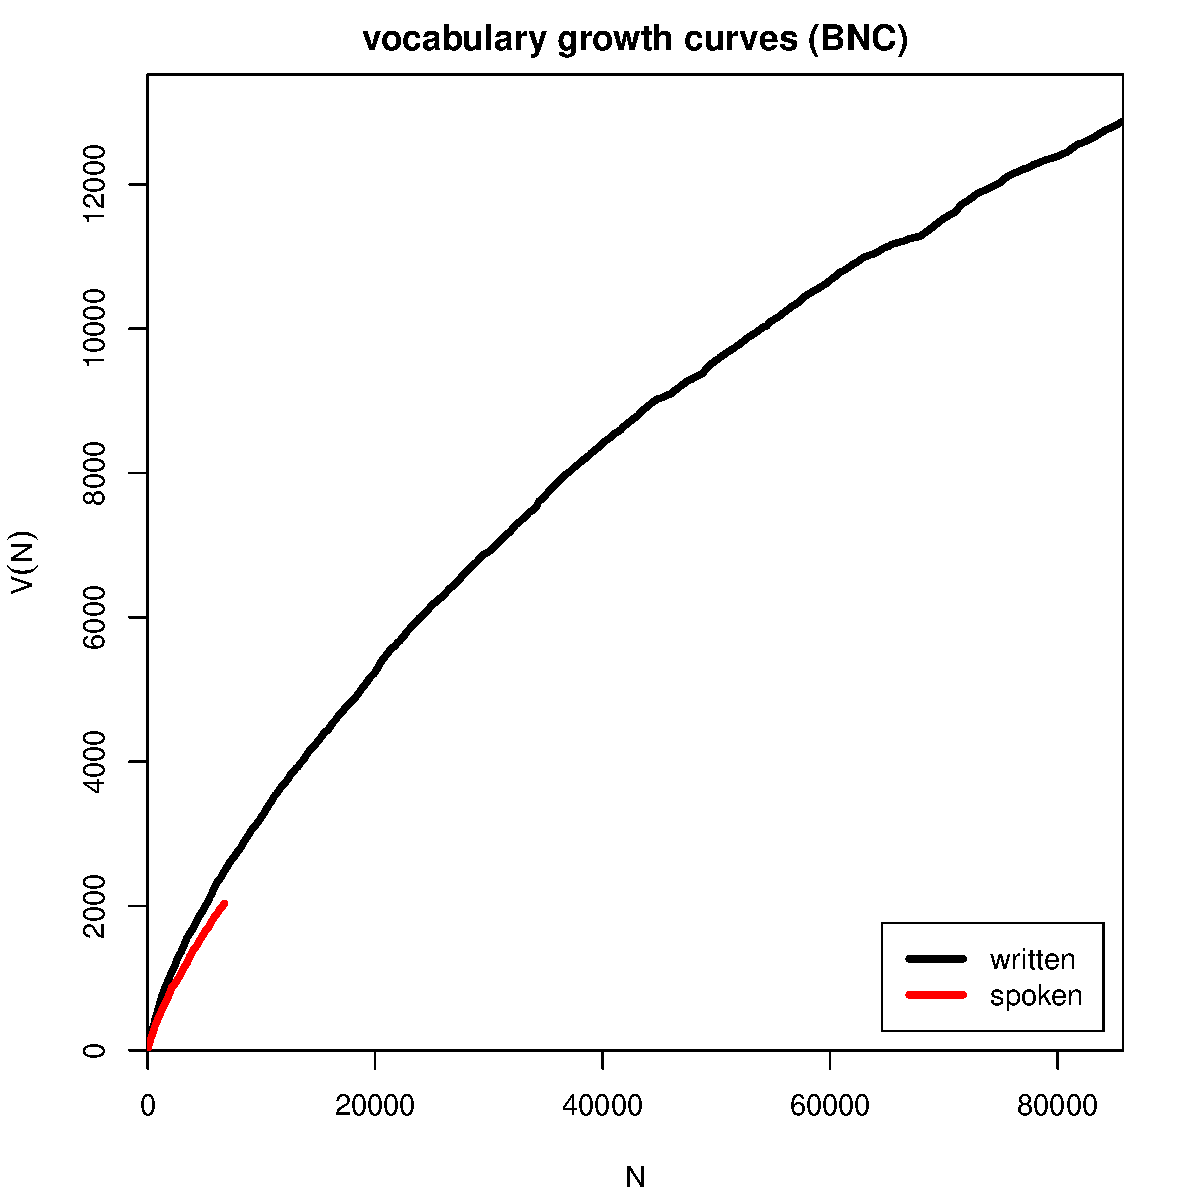
\includegraphics[width=6cm]{img/bare_bncWS_vgc}}
    \end{column}
  \end{columns}
\end{frame}

\begin{frame}[c]
  \frametitle{Are these ``lexical constants'' really constant?}
  %% \framesubtitle{}

  \centering
  \includegraphics[width=11cm]{img/bare_bncS_obs_lexical_constants}
\end{frame}

%%%%%%%%%%%%%%%%%%%%%%%%%%%%%%%%%%%%%%%%%%%%%%%%%%%%%%%%%%%%%%%%%%%%%%%%
\section{LNRE models}
\subsection{Population \& samples}

\begin{frame}
  \frametitle{LNRE models}

  \begin{itemize}
  \item State-of-the-art approach to measuring productivity:\\
    \h{LNRE models} \citep{Baayen:01}
    \begin{itemize}
    \item LNRE = Large Number of Rare Events
    \item \citet{Baayen:01} has 887 citations on Google Scholar
    \item[]
    \end{itemize}
  \item Standard implementation: \hh{zipfR} \citep{Evert:Baroni:07}
    \begin{itemize}
    \item 76 citations on Google Scholar
    \item only a few search results for Baayen's \texttt{lexstats} software
    \item[]
    \end{itemize}
  \item LNRE uses various approximations and simplifications to obtain a tractable and elegant model
    \begin{itemize}
    \item LNRE model usually minor component of complex procedure
    \item often applied to very large samples ($N > 1$ M tokens)
    \end{itemize}
  \end{itemize}
\end{frame}

\begin{frame}
  \frametitle{The LNRE population}

  \begin{itemize}
  \item Population: set of $S$ types $w_i$ with occurrence \h{probabilities} $\pi_i$
  \item $S$ = \h{population diversity} can be finite or infinite ($S = \infty$)
  \item Not interested in specific types \so  arrange by decreasing
    probability: $\pi_1\geq \pi_2\geq \pi_3 \geq \cdots$
    \begin{itemize}
    \item[\hand] impossible to determine probabilities of all individual types
    \end{itemize}
  \item Normalization: $\pi_1 + \pi_2 + \ldots + \pi_S = 1$
    \begin{itemize}
    \item[]
    \end{itemize}
  \item \hh{parametric} statistical \hh{model} to describe full population (esp.\ for $S = \infty$),
    i.e.\ a function $i \mapsto \pi_i$
    \begin{itemize}
    \item type probabilities $\pi_i$ cannot be estimated reliably from a sample, but parameters of this function can
    \item NB: population index $i$ $\neq$ Zipf rank $r$
    \end{itemize}
  \end{itemize}
\end{frame}

\begin{frame}
  \frametitle{Zipf-Mandelbrot law as a population model}

  \begin{itemize}
  \item Zipf-Mandelbrot law for type probabilities:
    \[ \pi_i := \frac{C}{(i + b) ^ a} \]
  \item Two free parameters: $a > 1$ and $b \geq 0$
    \begin{itemize}
    \item[\hand] $C$ is not a parameter but a normalization constant,\\
      needed to ensure that $\sum_i \pi_i = 1$
    \end{itemize}
  \item Third parameter: $S > 0$ or $S = \infty$
  \item[]
  \item This is the \h{Zipf-Mandelbrot} population model \citep{Evert:04}
  \end{itemize}
\end{frame}

\begin{frame}
  \frametitle{Samples: type frequency list \& spectrum}

  \ungap[1]
  \begin{center}
    \begin{tabular}[t]{r | rr}
      rank $r$ & $f_r$ & type $i$ \\
      \hline
       1 & 37 &  6 \\
       2 & 36 &  1 \\
       3 & 33 &  3 \\
       4 & 31 &  7 \\
       5 & 31 & 10 \\
       6 & 30 &  5 \\
       7 & 28 & 12 \\
       8 & 27 &  2 \\
       9 & 24 &  4 \\
      10 & 24 & 16 \\
      11 & 23 &  8 \\
      12 & 22 & 14 \\
      \vdots & \vdots & \vdots
    \end{tabular}
    \hspace{2cm}
    \begin{tabular}[t]{r | r}
      $m$ & $V_m$ \\
      \hline
       1 & 83 \\
       2 & 22 \\
       3 & 20 \\
       4 & 12 \\
       5 & 10 \\
       6 &  5 \\
       7 &  5 \\
       8 &  3 \\
       9 &  3 \\
      10 &  3 \\
      \vdots & \vdots \\
      \multicolumn{2}{c}{} \\
      \multicolumn{2}{c}{\hh{sample \#1}}
    \end{tabular}
  \end{center}
\end{frame}

\begin{frame}
  \frametitle{Samples: type frequency list \& spectrum}

  \ungap[1]
  \begin{center}
    \begin{tabular}[t]{r | rr}
      rank $r$ & $f_r$ & type $i$ \\
      \hline
       1 & 39 &  2 \\
       2 & 34 &  3 \\
       3 & 30 &  5 \\
       4 & 29 & 10 \\
       5 & 28 &  8 \\
       6 & 26 &  1 \\
       7 & 25 & 13 \\
       8 & 24 &  7 \\
       9 & 23 &  6 \\
      10 & 23 & 11 \\
      11 & 20 &  4 \\
      12 & 19 & 17 \\
      \vdots & \vdots & \vdots
    \end{tabular}
    \hspace{2cm}
    \begin{tabular}[t]{r | r}
      $m$ & $V_m$ \\
      \hline
       1 & 76 \\
       2 & 27 \\
       3 & 17 \\
       4 & 10 \\
       5 &  6 \\
       6 &  5 \\
       7 &  7 \\
       8 &  3 \\
      10 &  4 \\
      11 &  2 \\
      \vdots & \vdots \\
      \multicolumn{2}{c}{} \\
      \multicolumn{2}{c}{\hh{sample \#2}}
    \end{tabular}
  \end{center}
\end{frame}

\begin{frame}
  \frametitle{Expectation: frequency spectrum}

  \ungap[1]
  \begin{center}
    \only<beamer:0| handout:1>{%
      \begin{tabular}{cc}
        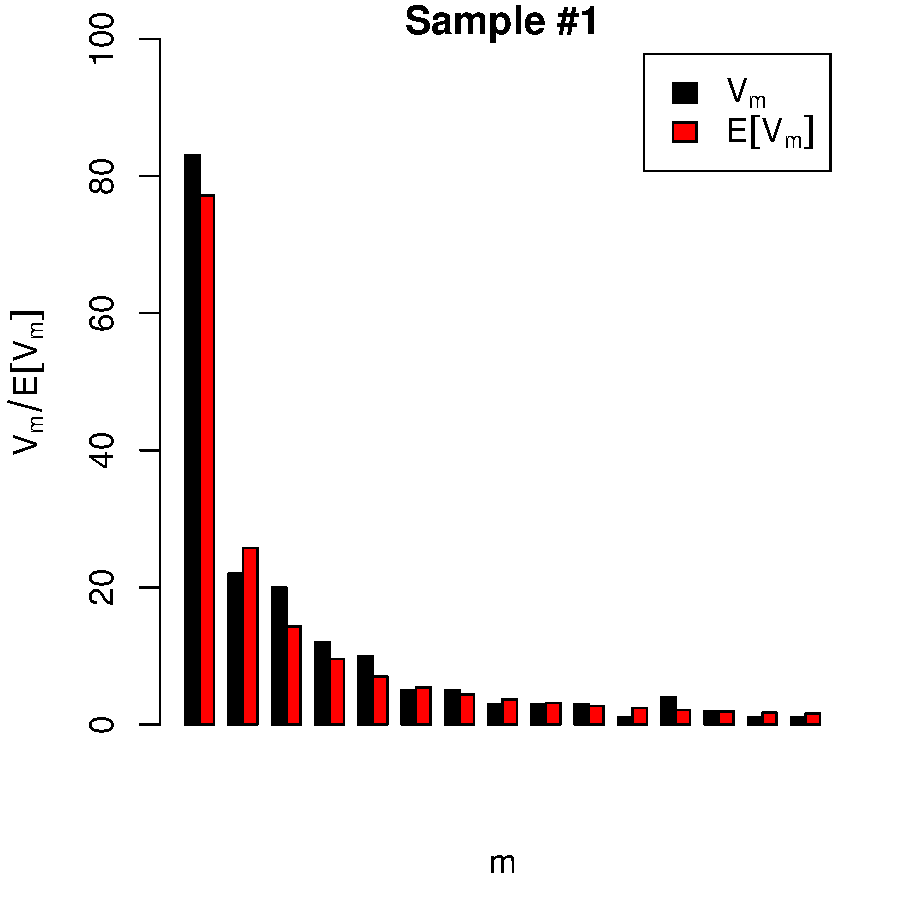
\includegraphics[width=40mm]{img/05-samples-spc-exp-vs-sample-1} &
        \includegraphics[width=40mm]{img/05-samples-spc-exp-vs-sample-2} \\
        \includegraphics[width=40mm]{img/05-samples-spc-exp-vs-sample-3} &
        \includegraphics[width=40mm]{img/05-samples-spc-exp-vs-sample-4} 
      \end{tabular}%
    }%
    \only<beamer:1| handout:0>{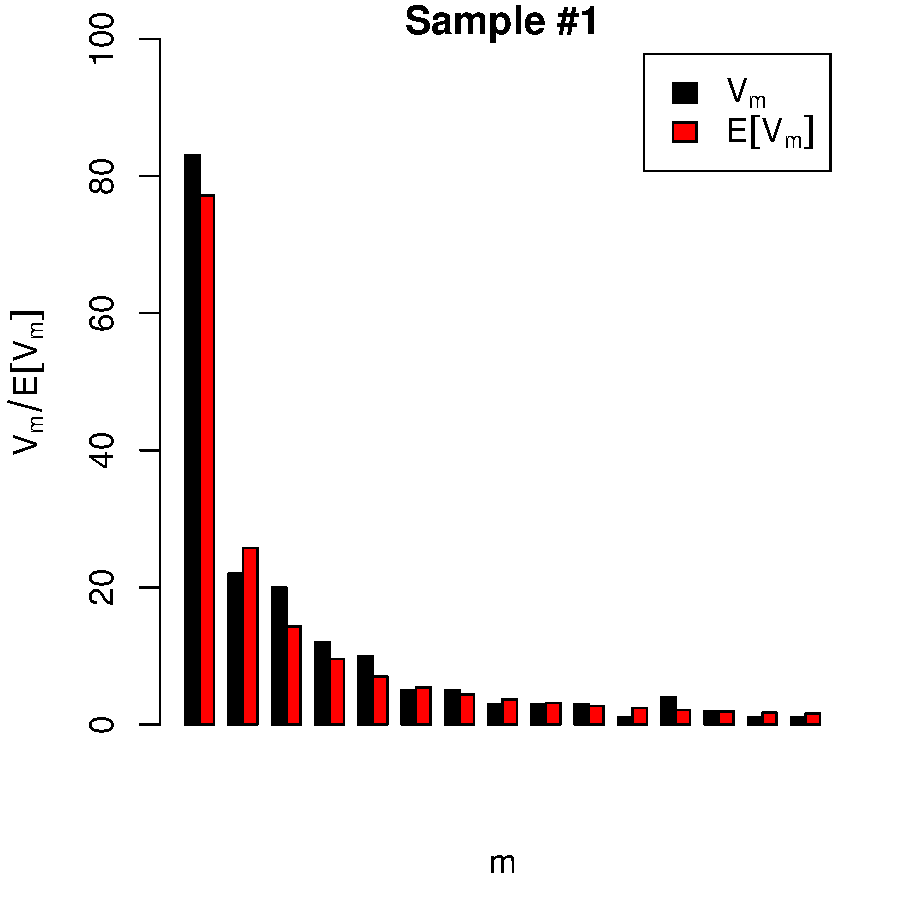
\includegraphics[width=70mm]{img/05-samples-spc-exp-vs-sample-1}}%
    \only<beamer:2| handout:0>{\includegraphics[width=70mm]{img/05-samples-spc-exp-vs-sample-2}}%
    \only<beamer:3| handout:0>{\includegraphics[width=70mm]{img/05-samples-spc-exp-vs-sample-3}}%
    \only<beamer:4| handout:0>{\includegraphics[width=70mm]{img/05-samples-spc-exp-vs-sample-4}}%
  \end{center}
\end{frame}

\begin{frame}
  \frametitle{Expectation: vocabulary growth curve}

  \ungap[1]
  \begin{center}
    \begin{tabular}{c @{} c}
      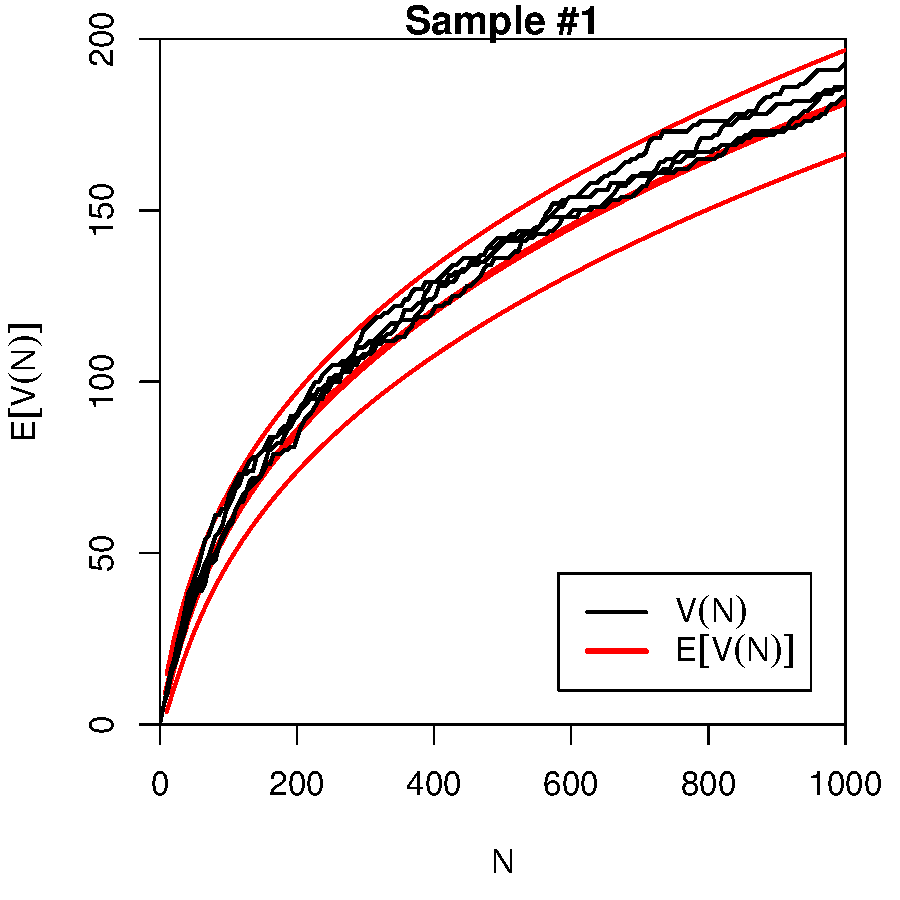
\includegraphics[width=50mm]{img/05-samples-vgc-exp-vs-samples-conf} &
      \includegraphics[width=50mm]{img/05-samples-vgc-V1-exp-vs-samples-conf}
    \end{tabular}
  \end{center}

  ``Confidence intervals'' indicate predicted sampling distribution:%
  \begin{itemize}
  \item[\hand] for 95\% of samples generated by the LNRE model, VGC will fall within the range delimited by the thin red lines
  \end{itemize}
\end{frame}

\begin{frame}[c]
  \frametitle{Extrapolating vocabulary growth}
  
  \centering
  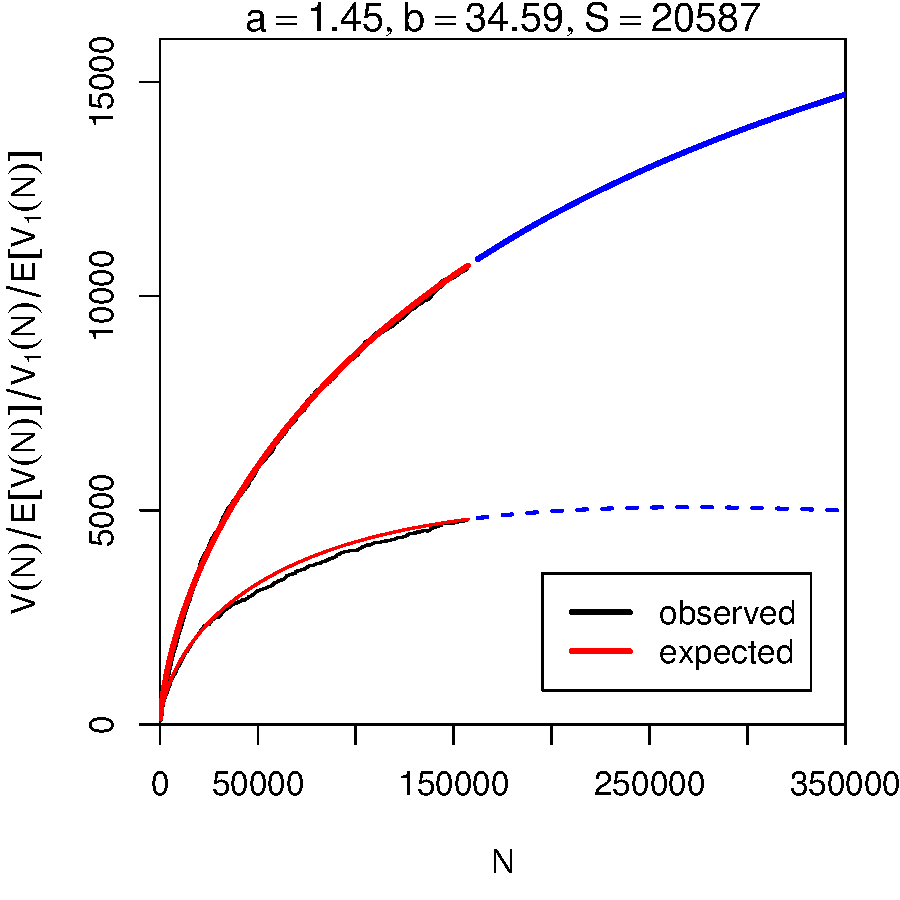
\includegraphics[width=7.5cm]{img/02-samples-ot-vgc-extrapolated}
\end{frame}

\begin{frame}<beamer:1-7| handout:0>
  \frametitle{Parameter estimation by trial \& error}

  \begin{center}
    \begin{tabular}{c @{} c}
      \only<beamer:1| handout:1>{\includegraphics[width=50mm]{img/05-estimation-spc-1}}%
      \only<beamer:2| handout:2>{\includegraphics[width=50mm]{img/05-estimation-spc-2}}%
      \only<beamer:3| handout:3>{\includegraphics[width=50mm]{img/05-estimation-spc-3}}%
      \only<beamer:4| handout:0>{\includegraphics[width=50mm]{img/05-estimation-spc-1}}%
      \only<beamer:5| handout:0>{\includegraphics[width=50mm]{img/05-estimation-spc-4}}%
      \only<beamer:6| handout:0>{\includegraphics[width=50mm]{img/05-estimation-spc-5}}%
      \only<beamer:7| handout:7>{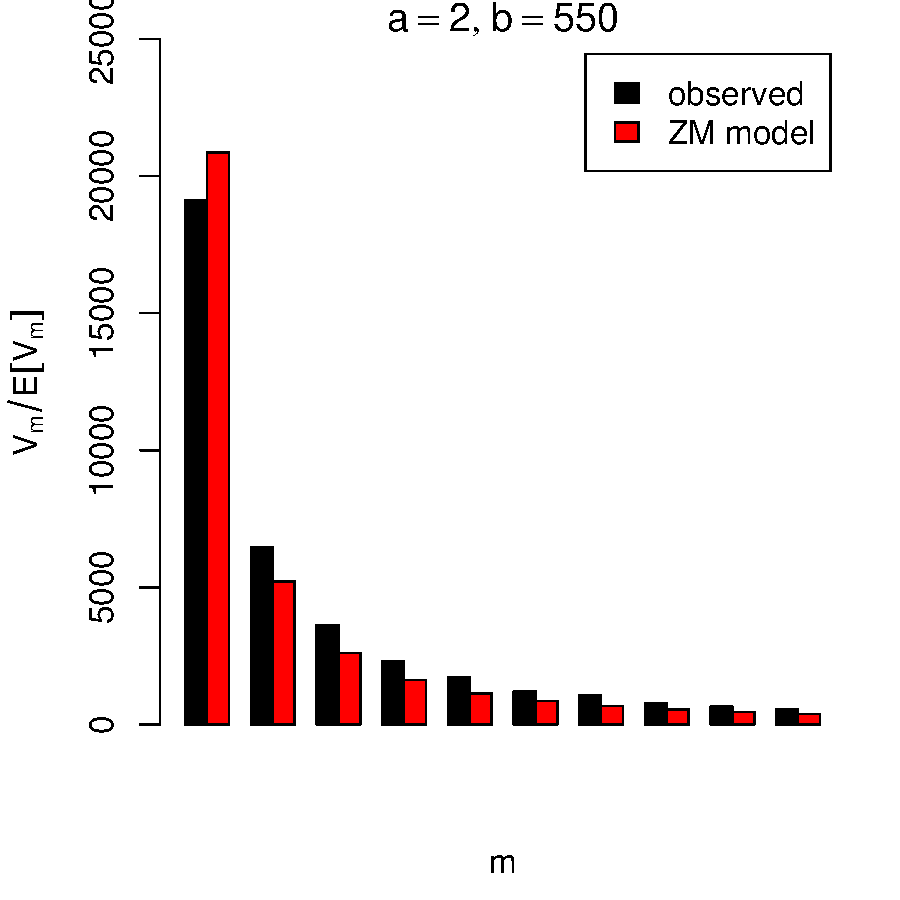
\includegraphics[width=50mm]{img/05-estimation-spc-6}}%
      &
      \only<beamer:1| handout:1>{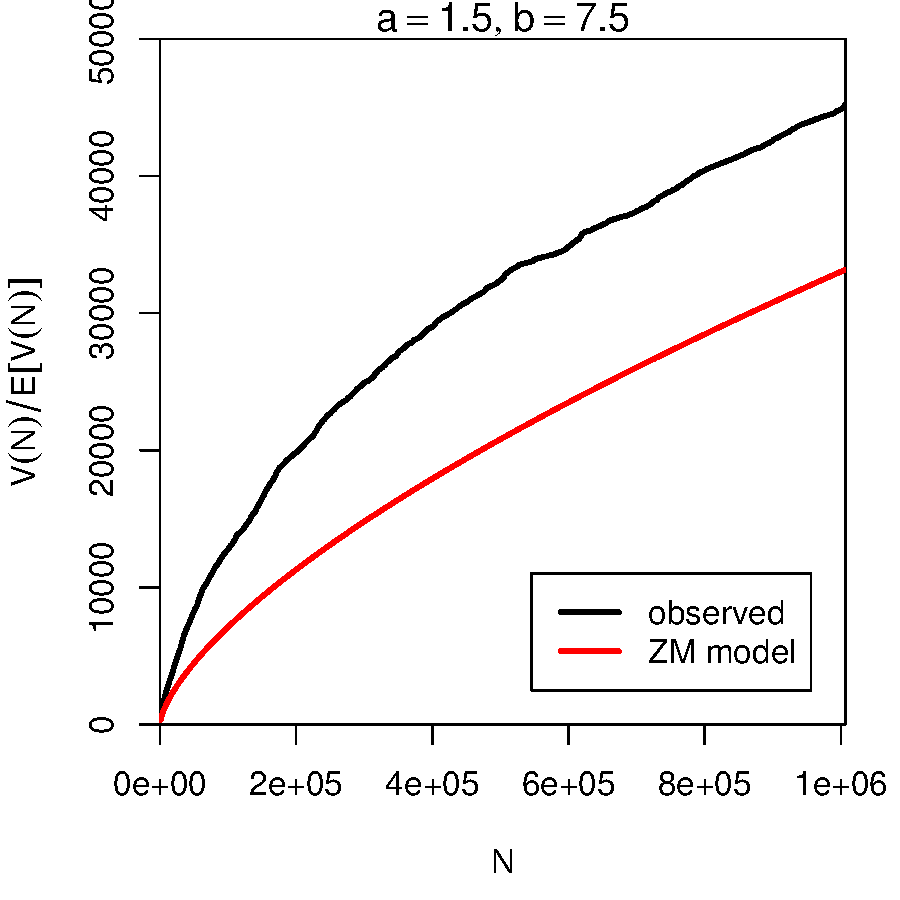
\includegraphics[width=50mm]{img/05-estimation-vgc-1}}%
      \only<beamer:2| handout:2>{\includegraphics[width=50mm]{img/05-estimation-vgc-2}}%
      \only<beamer:3| handout:3>{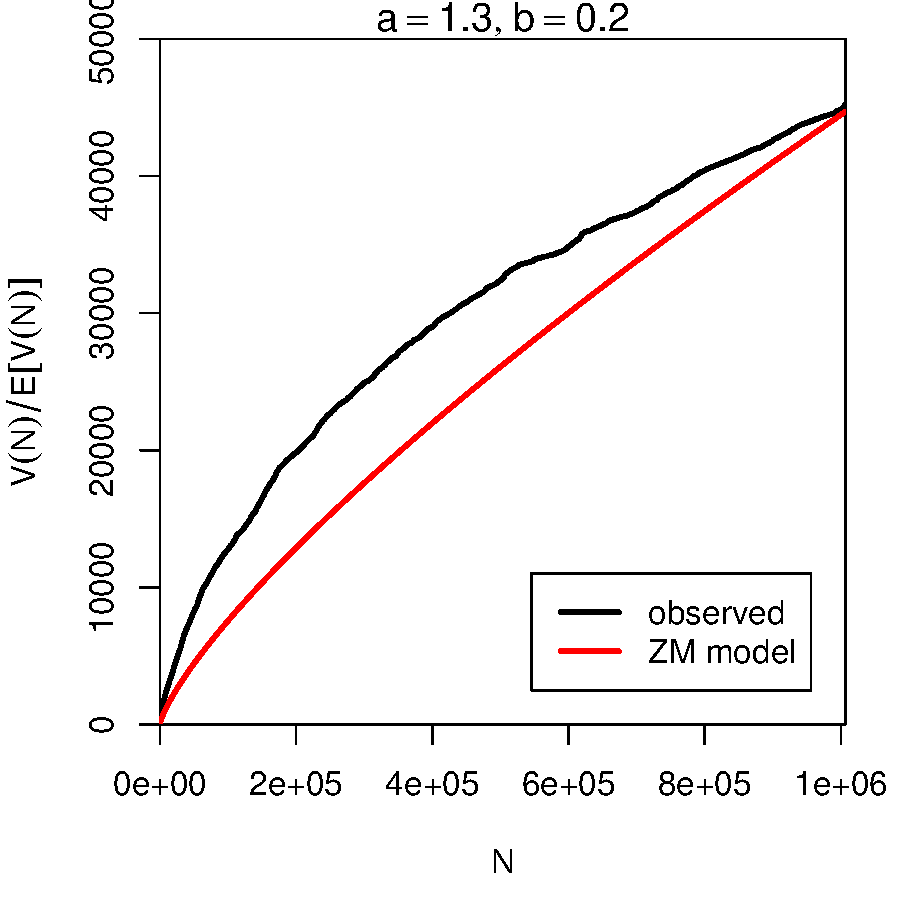
\includegraphics[width=50mm]{img/05-estimation-vgc-3}}%
      \only<beamer:4| handout:0>{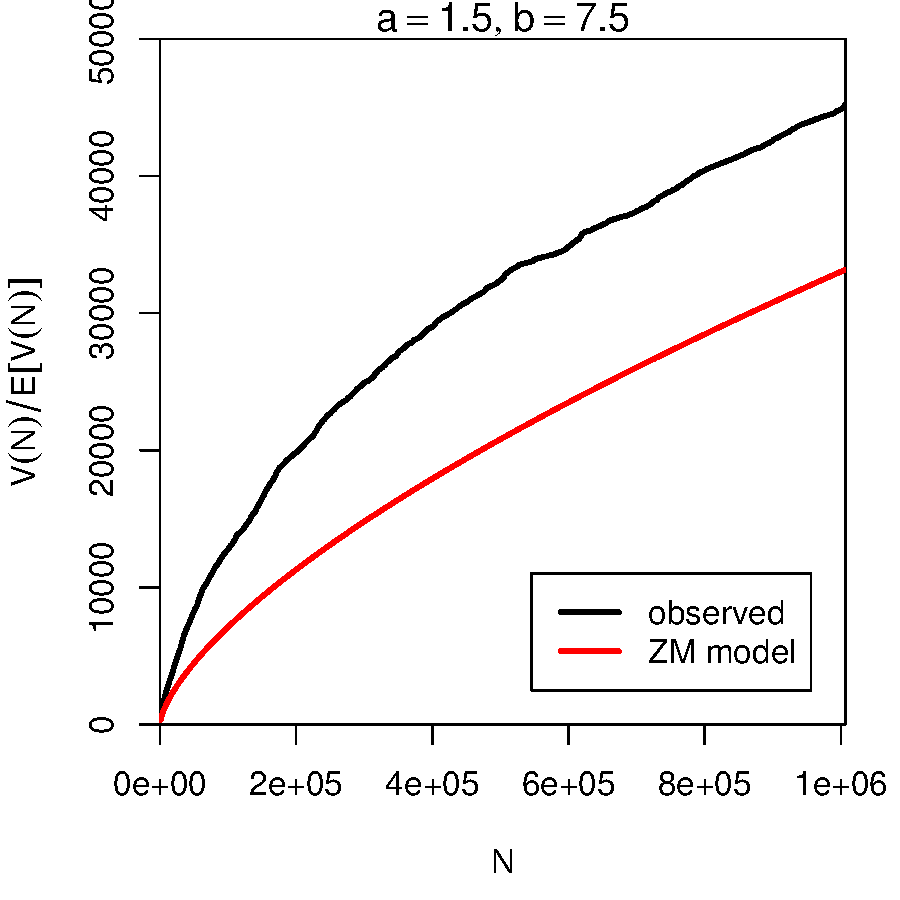
\includegraphics[width=50mm]{img/05-estimation-vgc-1}}%
      \only<beamer:5| handout:0>{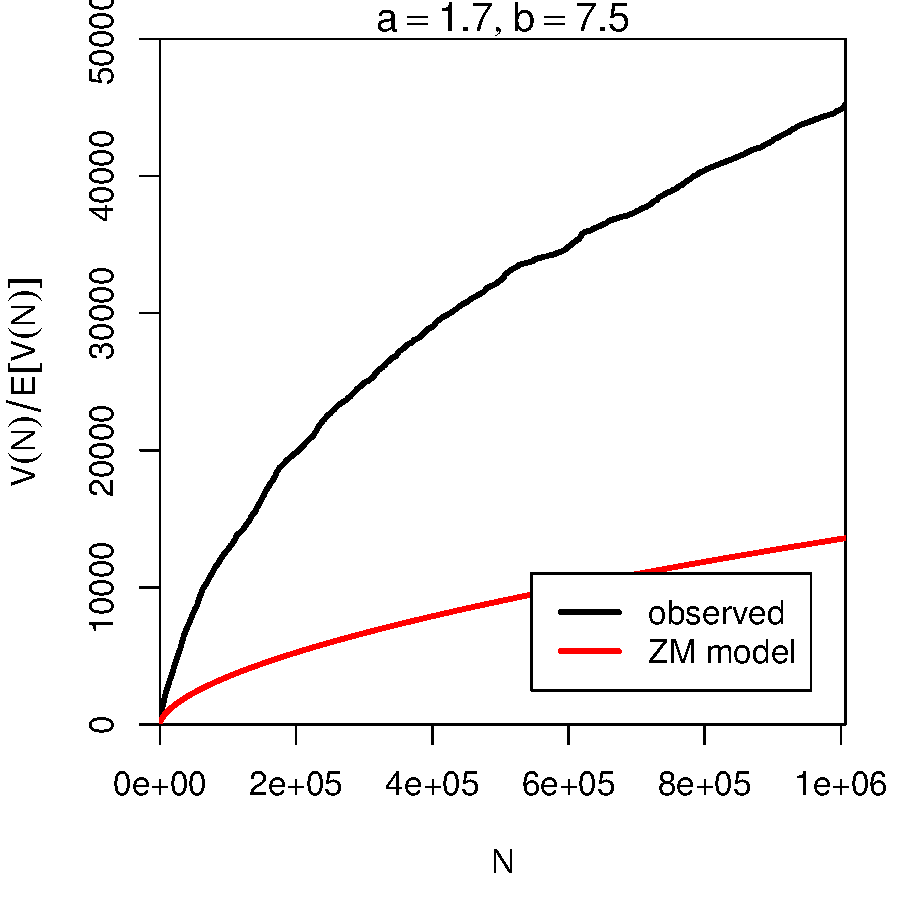
\includegraphics[width=50mm]{img/05-estimation-vgc-4}}%
      \only<beamer:6| handout:0>{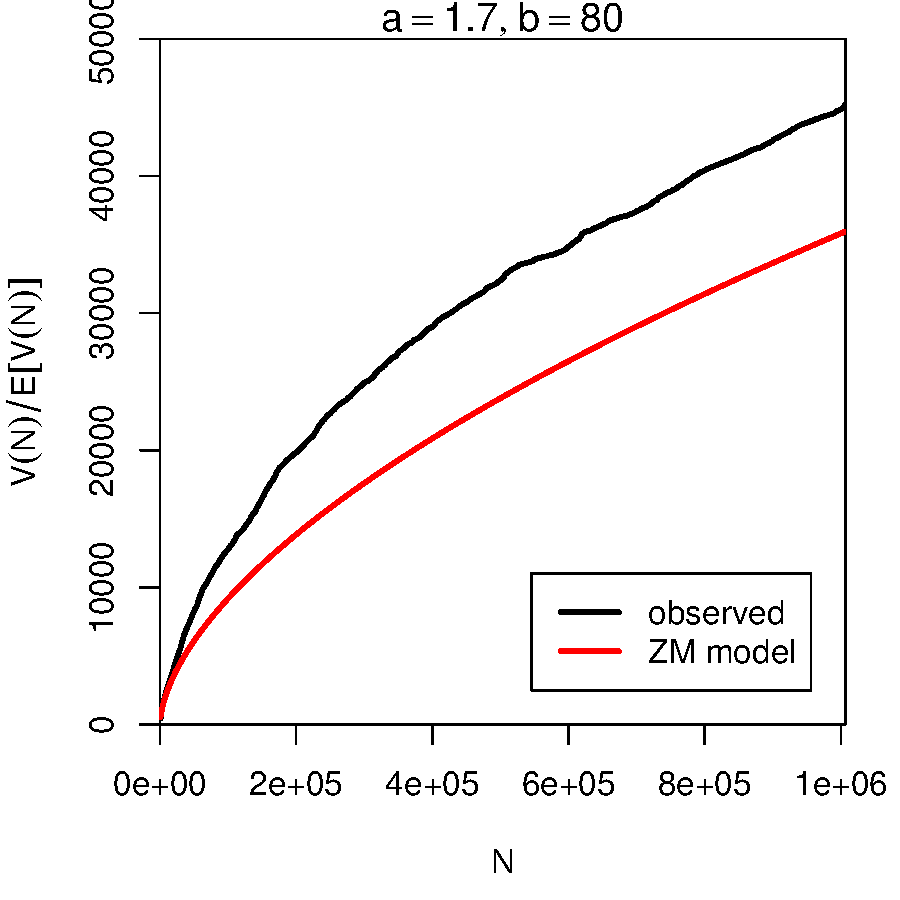
\includegraphics[width=50mm]{img/05-estimation-vgc-5}}%
      \only<beamer:7| handout:7>{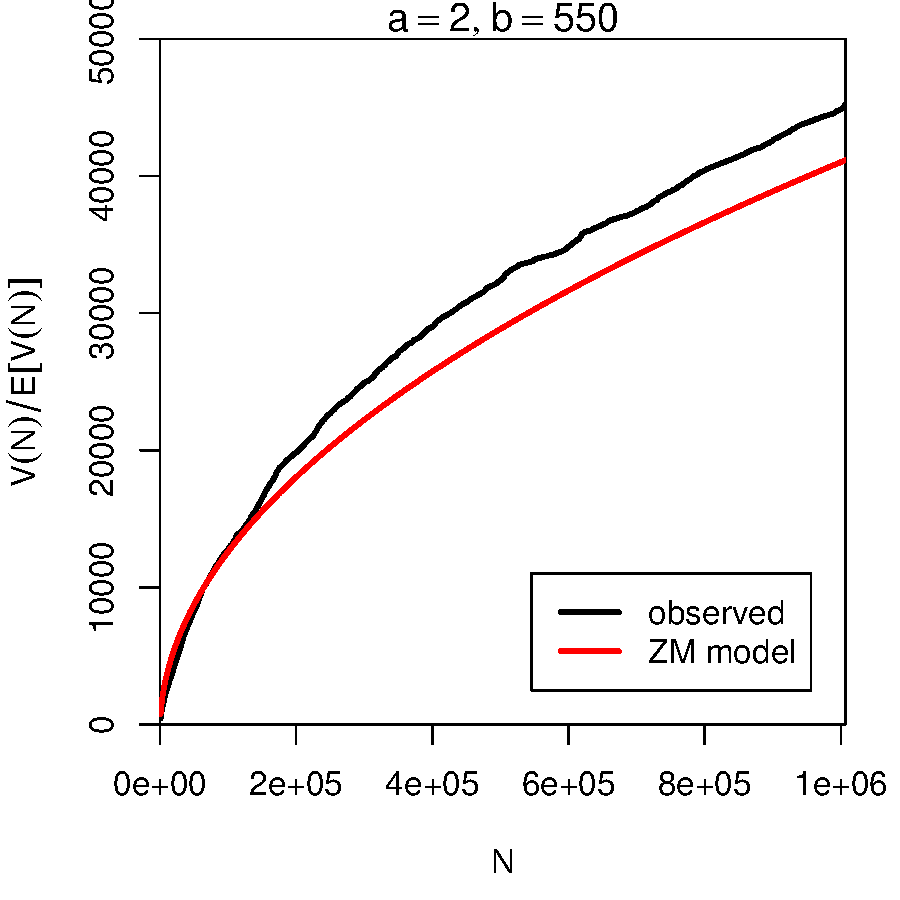
\includegraphics[width=50mm]{img/05-estimation-vgc-6}}%
    \end{tabular}
  \end{center}
\end{frame}

\begin{frame}[c]
  \frametitle{Parameter estimation}
  % \framesubtitle{Minimisation of suitable cost function for frequency spectrum}

  \begin{center}
    \begin{tabular}{c @{} c}
      \includegraphics[width=50mm]{img/05-estimation-spc-estimated} &
      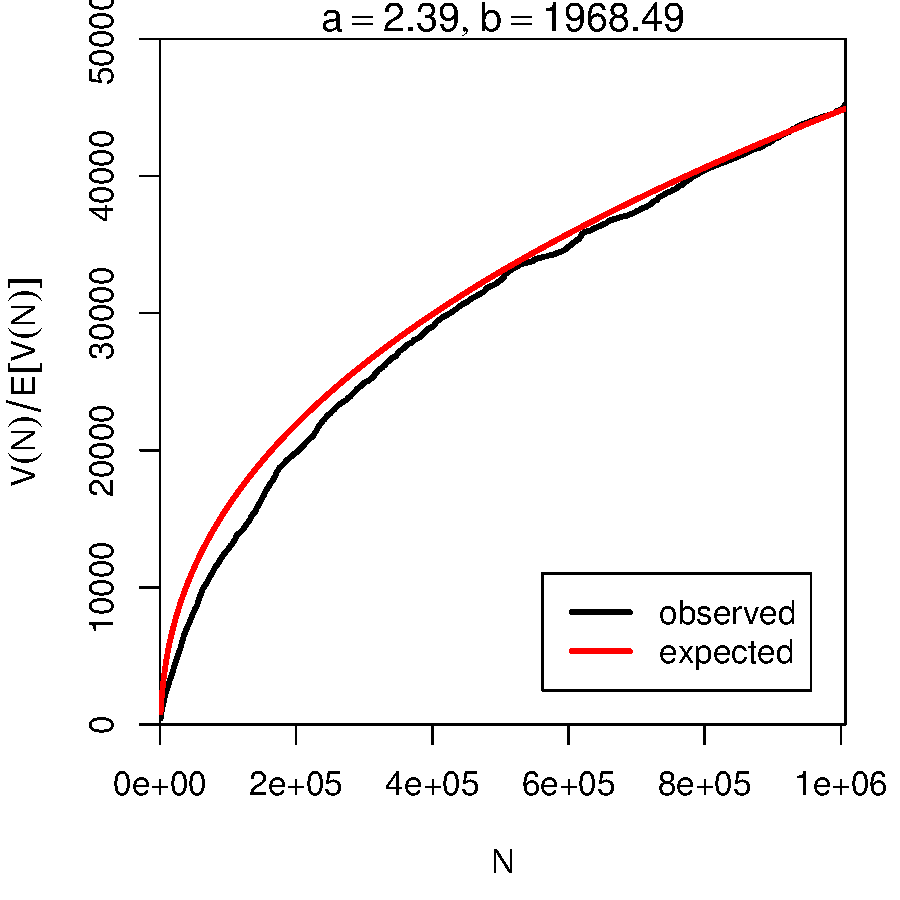
\includegraphics[width=50mm]{img/05-estimation-vgc-estimated} 
    \end{tabular}
  \end{center}

  \ungap[1]
  \begin{itemize}
    \item By trial \& error we found $a=2.0$ and $b=550$
    \item Automatic estimation procedure based on minimisation of suitable cost function: $a=2.39$ and $b=1968$
  \end{itemize}
\end{frame}

%%%%%%%%%%%%%%%%%%%%%%%%%%%%%%%%%%%%%%%%%%%%%%%%%%%%%%%%%%%%%%%%%%%%%%%%
\subsection{The mathematics of LNRE}

\begin{frame}
  \frametitle{The sampling model}

  \begin{itemize}
  \item Draw random sample of $N$ tokens from LNRE population
  \item Sufficient statistic: set of type frequencies $\set{f_i}$
    \begin{itemize}
    \item because tokens of random sample have no ordering
    \end{itemize}
  \item Joint \hh{multinomial} distribution of $\set{f_i}$:
    \[
      \pC{\set{f_i = k_i}}{N} =
      \frac{N!}{k_1! \cdots k_S!} \pi_1^{k_1} \cdots \pi_S^{k_S}
    \]
  \item<2-> \h{Approximation:} do not condition on fixed sample size $N$
    \begin{itemize}
    \item $N$ is now the average (expected) sample size
    \end{itemize}
  \item<2-> Random variables $f_i$ have \hh{independent Poisson} distributions:
    \[
      \p{f_i = k_i} = e^{-N\pi_i} \frac{(N\pi_i)^{k_i}}{k_i!}
    \]
  \end{itemize}
\end{frame}

\begin{frame}
  \frametitle{Frequency spectrum}

  \begin{itemize}
  \item Key problem: we cannot determine $f_i$ in observed sample
    \begin{itemize}
    \item because we don't know which type $w_i$ is
    \item recall that population ranking $f_i$ $\neq$ Zipf ranking $f_r$
    \end{itemize}
  \item Use spectrum $\set{V_m}$ and sample size $V$ as statistics
    \begin{itemize}
    \item contains all information we have about observed sample
    \end{itemize}
  \item<2-> Can be expressed in terms of indicator variables
    \begin{align*}
      \IV{f_i = m} &=
      \begin{cases}
        1 & f_i = m\\
        0 & \text{otherwise}
      \end{cases}\\
      \visible<3->{V_m &= \sum_{i=1}^S \IV{f_i = m}} \\
      \visible<4->{V &= \sum_{i=1}^S \IV{f_i > 0} = \sum_{i=1}^S \bigl( 1 - \IV{f_i = 0} \bigr)}
    \end{align*}
  \end{itemize}
\end{frame}

\begin{frame}
  \frametitle{The expected spectrum}

  \begin{itemize}
  \item It is easy to compute expected values for the frequency spectrum (and
    variances because the $f_i$ are independent)
    \begin{align*}
      \Exp{\IV{f_i = m}} &= \p{f_i = m} = e^{-N\pi_i} \frac{(N\pi_i)^m}{m!}\\
      \visible<2->{\Exp{V_m} &= \sum_{i=1}^S \Exp{\IV{f_i = m}} = \sum_{i=1}^S e^{-N\pi_i} \frac{(N\pi_i)^m}{m!}}\\
      \visible<3->{\Exp{V} &= \sum_{i=1}^S \bigExp{1 - \IV{f_i = 0}} = \sum_{i=1}^S \bigl( 1 - e^{-N\pi_i} \bigr)}
    \end{align*}
  \item<4-> NB: $V_m$ and $V$ are \primary{not independent} because they are
    derived from the same random variables $f_i$
  \end{itemize}
\end{frame}

\begin{frame}
  \frametitle{Sampling distribution of $V_m$ and $V$}

  \begin{itemize}
  \item Joint sampling distribution of $\set{V_m}$ and $V$ is complicated
  \item \h{Approximation:} $V$ and $\set{V_m}$ asymptotically follow a \hh{multivariate normal} distribution
    \begin{itemize}
    \item motivated by the multivariate central limit theorem:\\ sum of many independent variables $\IV{f_i = m}$
    \end{itemize}
  \item Usually limited to first spectrum elements, e.g.\ $V_1, \ldots, V_{15}$
    \begin{itemize}
    \item approximation of discrete $V_m$ by continuous distribution
      suitable only if $\Exp{V_m}$ is sufficiently large
    \end{itemize}
  \item<2-> Parameters of multivariate normal:
    $\pmb{\mu} = (\Exp{V}, \Exp{V_1}, \Exp{V_2}, \ldots)$ and $\pmb{\Sigma}$ = covariance matrix
    \[
      \bigp{(V, V_1, \ldots, V_k) = \mathbf{v}} \sim
      \frac{
        e^{-\frac12 (\mathbf{v} - \pmb{\mu})^T \pmb{\Sigma}^{-1} (\mathbf{v} - \pmb{\mu})}
      }{\small
        \sqrt{(2\pi)^{k+1} \det \pmb{\Sigma}}
      }
    \]
  \end{itemize}
\end{frame}

\begin{frame}
  \frametitle{Type density function}

  \begin{itemize}
  \item Discrete sums of probabilities in $\Exp{V}$, $\Exp{V_m}$, $\ldots$ are inconvenient and computationally expensive
  \item \h{Approximation:} continuous \h{type density function} $g(\pi)$
    \begin{align*}
      \abs{\setdef{w_i}{a \leq \pi_i \leq b}}
      &= \int_a^b g(\pi) \dpi\\
      \sum \setdef{\pi_i}{a \leq \pi_i \leq b}
      &= \int_a^b \pi g(\pi) \dpi
    \end{align*}
  \item<2-> Normalization constraint:
    \[
      \int_0^{\infty} \pi g(\pi) \dpi = 1
    \]
  \item<2-> Good approximation for low-probability types, but probability mass of $w_1, w_2, \ldots$ ``smeared out'' over range
  \end{itemize}
\end{frame}

\begin{frame}
  \frametitle{Type density function}

  \centering
  \begin{tikzpicture}
    \useasboundingbox (0, 0) rectangle (11, 7) ;
    \node[anchor=south west] at (0, 0) {\includegraphics[width=11cm]{../plots/lnre_tdf_vs_prob}} ;
    \visible<2->{
      \node[anchor=south west] at (4.5, 3) {\includegraphics[width=7cm]{../plots/lnre_pdf_vs_prob}} ;
    }
  \end{tikzpicture}
\end{frame}

\begin{frame}
  \frametitle{ZM and fZM as LNRE models}

  \begin{itemize}
  \item Discrete Zipf-Mandelbrot population
    \[
      \pi_i := \frac{C}{(i + b) ^ a} \quad \text{for } i = 1, \ldots, S
    \]
  \item<2-> Corresponding type density function \citep{Evert:04}
    \[
      g(\pi) =
      \begin{cases}
        C\cdot \pi^{-\alpha-1} & A \leq \pi \leq B\\
        0 & \text{otherwise}
      \end{cases}
    \]
    \onslide<3->
    with parameters
    \begin{itemize}
    \item $\primary{\alpha} = 1 / a$ ($0 < \alpha < 1$)
    \item $\primary{B} = b \cdot \alpha / (1 - \alpha)$
    \item $0 \leq \primary{A} < B$ determines $S$ (ZM with $S = \infty$ for $A = 0$)
    \item[\hand] $C$ is a normalization factor, not a parameter
    \end{itemize}
  \end{itemize}
\end{frame}

\begin{frame}[c]
  \frametitle{ZM and fZM as LNRE models}

  \centering
  \only<beamer:1| handout:0>{\includegraphics[width=11cm]{../plots/lnre_tdf_zm}}%
  \only<beamer:2| handout:1>{\includegraphics[width=11cm]{../plots/lnre_tdf_fzm}}%
\end{frame}

\begin{frame}
  \frametitle{Expectations as integrals}

  \begin{itemize}
  \item Expected values can now be expressed as integrals over $g(\pi)$
    \begin{align*}
      \Exp{V_m} &= \int_0^{\infty} \frac{(N\pi)^m}{m!} e^{-N\pi} g(\pi) \dpi\\
      \Exp{V} &= \int_0^{\infty} \bigl( 1 - e^{-N\pi} \bigr) g(\pi) \dpi
    \end{align*}
  \item<2-> Reduce to simple closed form for ZM (approximation)
    \begin{align*}
      \Exp{V_m} &= \frac{C}{m!} \cdot N^{\alpha} \cdot \Gamma (m - \alpha) \\
      \Exp{V} &= C \cdot N^{\alpha} \cdot \frac{\Gamma(1 - \alpha)}{\alpha}
    \end{align*}
  \item<2-> fZM (and exact solution for ZM) with incompl.\ Gamma function
  \end{itemize}
\end{frame}

\begin{frame}
  \frametitle{Parameter estimation from training corpus}

  \begin{itemize}
  \item For ZM, $\alpha = \frac{\Exp{V_1}}{\Exp{V}} \approx \frac{V_1}{V}$ can be estimated directly,\\
    but prone to overfitting
  \item General parameter fitting by \hh{MLE}:\\
    maximize likelihood of observed spectrum $\mathbf{v}$
    \[
      \max_{\alpha, A, B}\; \bigpC{(V, V_1, \ldots, V_k) = \mathbf{v}}{\alpha, A, B}
    \]
  \item<2-> Multivariate normal approximation:\\
    \[
      \min_{\alpha, A, B}\; (\mathbf{v} - \pmb{\mu})^T \pmb{\Sigma}^{-1} (\mathbf{v} - \pmb{\mu})
    \]
  \item<2-> Minimization by gradient descent (BFGS, CG) or simplex search (Nelder-Mead)
  \end{itemize}
\end{frame}

\begin{frame}[c]
  \frametitle{Parameter estimation from training corpus}

  \centering
  \only<beamer:1| handout:1>{\includegraphics[width=11cm]{img/cost_bncBare_chisq_10}}%
  \only<beamer:2| handout:0>{\includegraphics[width=11cm]{img/cost_brownWords_chisq_5}}%
\end{frame}

\begin{frame}
  \frametitle{Goodness-of-fit}
  \framesubtitle{\citep[Sec.~3.3]{Baayen:01}}

  \begin{itemize}
  \item How well does the fitted model explain the observed data?
  \item For multivariate normal distribution:
    \[
      X^2 = (\mathbf{V} - \pmb{\mu})^T \pmb{\Sigma}^{-1} (\mathbf{V} - \pmb{\mu}) \sim \chi^2_{k + 1}
    \]
    where $\mathbf{V} = (V, V_1, \ldots, V_k)$
  \item<2->[\So] Multivariate chi-squared test of \h{goodness-of-fit}
    \begin{itemize}
    \item replace $\mathbf{V}$ by observed $\mathbf{v}$ \so test statistic $x^2$
    \item must reduce $\text{df} = k + 1$ by number of estimated parameters
    \end{itemize}
  \item<2->[]
  \item<2-> NB: significant rejection of the LNRE model for $p < .05$
  \end{itemize}
\end{frame}

%%%%%%%%%%%%%%%%%%%%%%%%%%%%%%%%%%%%%%%%%%%%%%%%%%%%%%%%%%%%%%%%%%%%%%%%

\logo{\includegraphics[width=4cm]{img/Macchiato}}
\begin{frame}[c]
  \begin{center}
    \counterpoint{\huge Coffee break?}
  \end{center}
\end{frame}
\hideLogo{}


%%%%%%%%%%%%%%%%%%%%%%%%%%%%%%%%%%%%%%%%%%%%%%%%%%%%%%%%%%%%%%%%%%%%%%%% 
\section{Problems}

%%%%%%%%%%%%%%%%%%%%%%%%%%%%%%%%%%%%%%%%%%%%%%%%%%%%%%%%%%%%%%%%%%%%%%%%
\subsection{Interpretability of measures}

\begin{frame}[c]
  \frametitle{Empirical observations}
  %% \framesubtitle{}

  \centering
  \includegraphics[width=11cm]{img/bare_bncS_obs_lexical_constants}
\end{frame}

\begin{frame}
  \frametitle{Parametric bootstrapping with LNRE models}

  \begin{columns}[T]
    \begin{column}{55mm}
      \begin{itemize}
      \item Use simulation experiments to gain better understanding of quantitative measures
      \item Resampling (bootstrapping) leads to biased type counts
      \item<2->[\So] Parametric bootstrapping based on LNRE population
        \begin{itemize}
        \item arbitrary sample size
        \item intuitive notion of productivity \so parameters 
        \item controlled manipulation of confounding factors
        \end{itemize}
      \end{itemize}
    \end{column}
    \begin{column}{45mm}
      \visible<2->{\includegraphics[width=45mm]{img/lexconst_spectra}}%
    \end{column}
  \end{columns}
\end{frame}

\begin{frame}[c]
  \frametitle{Parametric bootstrapping: sample size}
  
  \centering
  \includegraphics[width=11cm]{img/lexconst_sample_size}
\end{frame}

\begin{frame}[c]
  \frametitle{Parametric bootstrapping: frequent lexicalized types}

  \centering
  \includegraphics[width=11cm]{img/lexconst_echo_type}
\end{frame}


%%%%%%%%%%%%%%%%%%%%%%%%%%%%%%%%%%%%%%%%%%%%%%%%%%%%%%%%%%%%%%%%%%%%%%%%
\subsection{LNRE models}

\begin{frame}
  \frametitle{Problems of LNRE models}

  \ungap[1]
  \begin{itemize}
  \item Assumption: corpus data = random sample
    \begin{itemize}
    \item[\hand] holds reasonably well for morphological productivity
    \item[\hand] simple but effective \textsc{echo} correction \citep{Baroni:Evert:07a}
    \item[]
    \end{itemize}
  \item<2-> Approximation: independent Poisson sampling
    \begin{itemize}
    \item instead of correct multinomial sampling distribution
    \item[]
    \end{itemize}
  \item<3-> Approximation: multivariate normal distribution of $V$ and $V_m$
    \begin{itemize}
    \item true sampling distribution is completely intractable
    \item[]
    \end{itemize}
  \item<4-> Approximation: continuous type density function $g(\pi)$
    \begin{itemize}
    \item instead of discrete type probabilities of Z-M law
    \item[]
    \end{itemize}
  \item[\So]<5-> Wide-spread irresponsible application of LNRE models to small samples \citep[e.g.][]{Luedeling:Evert:05}
  \end{itemize}
\end{frame}

\begin{frame}
  \frametitle{How reliable are the fitted models?}
  
  Three potential issues:
  \begin{enumerate}
  \item<2-> \h<5->{Model assumptions $\neq$ population}\\
    (e.g.\ distribution does not follow a Zipf-Mandelbrot law)
    \begin{itemize}
    \item[\hand] model cannot be adequate, regardless of parameter settings
    \item[]
    \end{itemize}
  \item<3-> \h<5->{Parameter estimation unsuccessful}\\
    (i.e.\ suboptimal goodness-of-fit to training data)
    \begin{itemize}
    \item[\hand] optimization algorithm trapped in local minimum
    \item[\hand] can result in highly inaccurate model
    \item[]
    \end{itemize}
  \item<4-> Uncertainty due to sampling variation\\
    (i.e.\ training data differ from population distribution)
    \begin{itemize}
    \item[\hand] model fitted to training data, may not reflect true population
    \item[\hand] another training sample would have led to different parameters
    \item[\hand] especially critical for small samples ($N < $ 10,000)
    \end{itemize}
  \end{enumerate}
\end{frame}

\begin{frame}[c]
  \frametitle{Cost functions for German word-formation affixes}

  \centering
  \only<beamer:1| handout:0>{\includegraphics[height=7.5cm]{../plots/cost_bar_linear_m10}}%
  \only<beamer:2| handout:0>{\includegraphics[height=7.5cm]{../plots/cost_bar_mse_m10}}%
  \only<beamer:3| handout:0>{\includegraphics[height=7.5cm]{../plots/cost_bar_chi-square_m10}}%
  \only<beamer:4| handout:0>{\includegraphics[height=7.5cm]{../plots/cost_bar_MLE_m10}}%
  \only<beamer:5| handout:0>{\includegraphics[height=7.5cm]{../plots/cost_bar_MLE_m05}}%
  \only<beamer:6| handout:0>{\includegraphics[height=7.5cm]{../plots/cost_chen_MLE_m05}}%
  \only<beamer:7| handout:0>{\includegraphics[height=7.5cm]{../plots/cost_lein_MLE_m05}}%
  \only<beamer:8| handout:0>{\includegraphics[height=7.5cm]{../plots/cost_sam_MLE_m05}}%
  \only<beamer:0| handout:1>{%
    \hspace*{-5mm}%
    \begin{tabular}{c@{}c}
      \includegraphics[height=6cm]{../plots/cost_bar_mse_m10}
      & \includegraphics[height=6cm]{../plots/cost_bar_MLE_m05}
    \end{tabular}%
  }

\end{frame}

%%%%%%%%%%%%%%%%%%%%%%%%%%%%%%%%%%%%%%%%%%%%%%%%%%%%%%%%%%%%%%%%%%%%%%%%
\subsection{Confidence intervals}

\begin{frame}
  \frametitle{Goodness-of-fit}
  \framesubtitle{\citep[Sec.~3.3]{Baayen:01}}

  \begin{itemize}
  \item Statistics: confidence intervals for population coefficients by inverting hypothesis tests (all $H_0: \mu = x$ with $p > .05$)
  \item<2-> Multivariate normal approximation for $\mathbf{V} = (V, V_1, \ldots, V_k)$:
    \[
      \bigp{\mathbf{V} = \mathbf{v}} \sim
      \frac{
        e^{-\frac12 (\mathbf{v} - \pmb{\mu})^T \pmb{\Sigma}^{-1} (\mathbf{v} - \pmb{\mu})}
      }{\small
        \sqrt{(2\pi)^{k+1} \det \pmb{\Sigma}}
      }
    \]
    with $\pmb{\mu} = (\Exp{V}, \Exp{V_1}, \Exp{V_2}, \ldots)$ and $\pmb{\Sigma}$ = covariance matrix
  \item[]
  \item<3-> Test statistic
    \[
      X^2 = (\mathbf{V} - \pmb{\mu})^T \pmb{\Sigma}^{-1} (\mathbf{V} - \pmb{\mu}) \sim \chi^2_{k + 1}
    \]
  \item<3->[\So] Multivariate chi-squared test of \h{goodness-of-fit}
    \begin{itemize}
    \item[\hand] significant rejection of the LNRE model for $p < .05$
    \end{itemize}
  \end{itemize}
\end{frame}

\begin{frame}[c]
  \frametitle{Confidence sets based on goodness-of-fit test?}

  \centering
  \only<beamer:1| handout:0>{\includegraphics[height=7.5cm]{../plots/cost_lein_MLE_m05}}%
  \only<beamer:2| handout:0>{\includegraphics[height=7.5cm]{../plots/gof_lein_m05}}%
  \only<beamer:3| handout:0>{\includegraphics[height=7.5cm]{../plots/cost_bar_MLE_m05}}%
  \only<beamer:4| handout:0>{\includegraphics[height=7.5cm]{../plots/gof_bar_m05}}%
  \only<beamer:5| handout:0>{\includegraphics[height=7.5cm]{../plots/cost_sam_MLE_m05}}%
  \only<beamer:6| handout:0>{\includegraphics[height=7.5cm]{../plots/gof_sam_m05}}%
  \only<beamer:0| handout:1>{%
    \hspace*{-5mm}%
    \begin{tabular}{c@{}c}
      \includegraphics[height=6cm]{../plots/cost_lein_MLE_m05}
      & \includegraphics[height=6cm]{../plots/gof_lein_m05}
    \end{tabular}%
  }%
  \only<beamer:0| handout:2>{%
    \hspace*{-5mm}%
    \begin{tabular}{c@{}c}
      \includegraphics[height=6cm]{../plots/cost_sam_MLE_m05}
      & \includegraphics[height=6cm]{../plots/gof_sam_m05}
    \end{tabular}%
  }%
\end{frame}

\begin{frame}[c]
  \frametitle{Confidence sets for idealized samples from ZM population}
  \framesubtitle{\primary{\so $X^2$ tests model parameters rather than goodness-of-fit}}

  \centering\ungap[.5]
  \only<beamer:1| handout:0>{\includegraphics[height=7.5cm]{../plots/gof_zm_spc_1000000}}%
  \only<beamer:2| handout:0>{\includegraphics[height=7.5cm]{../plots/gof_zm_spc_50000}}%
  \only<beamer:3| handout:0>{\includegraphics[height=7.5cm]{../plots/gof_zm_spc_10000}}%
  \only<beamer:4| handout:0>{\includegraphics[height=7.5cm]{../plots/gof_zm_spc_5000}}%
  \only<beamer:5| handout:0>{\includegraphics[height=7.5cm]{../plots/gof_zm_spc_2000}}%
  \only<beamer:6| handout:0>{\includegraphics[height=7.5cm]{../plots/gof_zm_spc_1000}}%
  \only<beamer:7| handout:0>{\includegraphics[height=7.5cm]{../plots/gof_zm_spc_500}}%
  \only<beamer:8| handout:0>{\includegraphics[height=7.5cm]{../plots/gof_zm_spc_200}}%
  \only<beamer:0| handout:1>{%
    \hspace*{-5mm}%
    \begin{tabular}{c@{}c}
      \includegraphics[height=6cm]{../plots/gof_zm_spc_5000}
      & \includegraphics[height=6cm]{../plots/gof_zm_spc_200}
    \end{tabular}%
  }%
\end{frame}

%%%%%%%%%%%%%%%%%%%%%%%%%%%%%%%%%%%%%%%%%%%%%%%%%%%%%%%%%%%%%%%%%%%%%%%%%%%%%
\subsection{Bootstrapping}

\begin{frame}
  \frametitle{How reliable are the fitted models?}
  
  Three potential issues:
  \begin{enumerate}
  \item Model assumptions $\neq$ population\\
    (e.g.\ distribution does not follow a Zipf-Mandelbrot law)
    \begin{itemize}
    \item[\hand] model cannot be adequate, regardless of parameter settings
    \item[]
    \end{itemize}
  \item Parameter estimation unsuccessful\\
    (i.e.\ suboptimal goodness-of-fit to training data)
    \begin{itemize}
    \item[\hand] optimization algorithm trapped in local minimum
    \item[\hand] can result in highly inaccurate model
    \item[]
    \end{itemize}
  \item \h{Uncertainty due to sampling variation}\\
    (i.e.\ training data differ from population distribution)
    \begin{itemize}
    \item[\hand] model fitted to training data, may not reflect true population
    \item[\hand] another training sample would have led to different parameters
    \item[\hand] especially critical for small samples ($N < $ 10,000)
    \end{itemize}
  \end{enumerate}
\end{frame}

\begin{frame}
  \frametitle{Bootstrapping}

  \begin{itemize}
  \item<1-> An empirical approach to sampling variation:
    \begin{itemize}
    \item take many random samples from the same population
    \item estimate LNRE model from each sample
    \item analyse distribution of model parameters, goodness-of-fit, etc.
      (mean, median, s.d., boxplot, histogram, \ldots)
    \item problem: how to obtain the additional samples?
    \end{itemize}
  \item<2-> Bootstrapping \citep{Efron:79}
    \begin{itemize}
    \item resample from observed data \emph{with replacement}
    \item this approach is not suitable for type-token distributions
      (resamples underestimate vocabulary size $V$!)
    \end{itemize}
  \item<3-> Parametric bootstrapping
    \begin{itemize}
    \item use fitted model to generate samples, i.e.\ sample from the population described by the model
    \item advantage: ``correct'' parameter values are known
    \end{itemize}
  \end{itemize}
\end{frame}

\begin{frame}
  \frametitle{Bootstrapping}
  \framesubtitle{parametric bootstrapping with 100 replicates, fZM samples for $N = 3467$}

  \ungap[.5]
  \only<beamer:1| handout:1>{\h{Zipfian slope $a = 1 / \alpha$}}%
  \only<beamer:2| handout:0>{\h{Offset $b = (1 - \alpha) / (B\cdot \alpha)$}}%
  \only<beamer:3| handout:0>{\h{fZM probability cutoff $A = \pi_S$}}%
  \only<beamer:4| handout:2>{\h{Goodness-of-fit statistic $X^2$} \secondary{(model not plausible for $X^2 > 11$)}}%
  \only<beamer:5-6| handout:3>{\h{Population diversity $S$}}%
  \ungap[.5]
  \begin{center}
    \only<beamer:1| handout:1>{\includegraphics[width=10cm]{img/05-bootstrap-ultra-alpha}}%
    \only<beamer:2| handout:0>{\includegraphics[width=10cm]{img/05-bootstrap-ultra-B}}%
    \only<beamer:3| handout:0>{\includegraphics[width=10cm]{img/05-bootstrap-ultra-A}}%
    \only<beamer:4| handout:2>{\includegraphics[width=10cm]{img/05-bootstrap-ultra-X2}}%
    \only<beamer:5| handout:0>{\includegraphics[width=10cm]{img/05-bootstrap-ultra-S}}%
    \only<beamer:6| handout:3>{\includegraphics[width=10cm]{img/05-bootstrap-ultra-S-zoomed}}%
  \end{center}
\end{frame}

\begin{frame}[c]
  \frametitle{Sample size matters!}
  \framesubtitle{Brown corpus is too small for reliable LNRE parameter estimation (bare singulars)}

  \centering
  \includegraphics[width=11cm]{img/bare_brown_boot_fzm_a_S}
\end{frame}

%%%%%%%%%%%%%%%%%%%%%%%%%%%%%%%%%%%%%%%%%%%%%%%%%%%%%%%%%%%%%%%%%%%%%%%%%%%%%
\subsection{Research programme}

\begin{frame}
  \frametitle{My research programme for LNRE models}

  \begin{itemize}
  \item<1-> Improve efficiency \& numerical accuracy of implementation
    \begin{itemize}
    \item numerical integrals instead of differences of Gamma functions
    \item efficient generation of large random samples
    \end{itemize}
  \item<2-> Analyze accuracy of LNRE approximations
    \begin{itemize}
    \item comprehensive simulation experiments, esp.\ for small samples
    \end{itemize}
  \item<3-> Specify more flexible LNRE population models
    \begin{itemize}
    \item my favourite: piecewise Zipfian type density functions
    \item flexible approximation, but no deep mathematical justification
    \end{itemize}
  \item<4-> Develop hypothesis tests \& confidence intervals
    \begin{itemize}
    \item key challenge: goodness-of-fit \vs confidence region
    \item prediction intervals for model-based extrapolation
    \end{itemize}
  \item<5-> Simulation experiments for productivity measures
    \begin{itemize}
    \item Can we find a quantitative measure that is robust against confounding factors and corresponds to intuitive notions of productivity \& lexical diversity?
    \end{itemize}
  \end{itemize}
\end{frame}

\begin{frame}
  \frametitle{My research programme for LNRE models}

  \begin{itemize}
  \item<1-> Is non-randomness a problem?
    \begin{itemize}
    \item not for morphological productivity \so \textsc{echo} correction
    \item tricky to include explicitly in LNRE approach
    \item[]
    \end{itemize}
  \item<2-> Do we need LNRE models for practical applications?
    \begin{itemize}
    \item better productivity measures + empirical sampling variation
    \item e.g.\ by cross-validation \citep{Evert:Wankerl:Noeth:17}
    \item[]
    \end{itemize}
  \item<3-> How important is semantics \& context?
    \begin{itemize}
    \item Does it make sense to measure productivity and lexical diversity purely in terms of type-token distributions?
    \item e.g.\ register variation for morphological productivity
    \item type-token ratio $\neq$ complexity of author's vocabulary
    \end{itemize}
  \end{itemize}
\end{frame}

%%%%%%%%%%%%%%%%%%%%%%%%%%%%%%%%%%%%%%%%%%%%%%%%%%%%%%%%%%%%%%%%%%%%%% 

\begin{frame}[c]
  \begin{center}
    \counterpoint{\huge Thank you!}
  \end{center}
\end{frame}


%%%%%%%%%%%%%%%%%%%%%%%%%%%%%%%%%%%%%%%%%%%%%%%%%%%%%%%%%%%%%%%%%%%%%%
%% References (if any)

\frame[allowframebreaks]{
  \frametitle{References}
  \bibliographystyle{natbib-stefan}
  \begin{scriptsize}
    \bibliography{stefan-publications,stefan-literature}
  \end{scriptsize}
}

\end{document}
